\documentclass{article}
\usepackage{graphicx} % Required for inserting images
\graphicspath{{Figures/}} % look for images in the Figures/ folder
\usepackage{amsmath}
\usepackage[hidelinks]{hyperref} % clickable hyperlinks (hidelinks = no visual change to existing refs)
\title{Analytical DOS derivation for CNTs}
\author{Shlok Vaibhav Singh }
\date{August 2026}


\begin{document}

\maketitle

\begin{abstract}
In this tutorial, we derive analytically the density of states for a CNT tube that matches 
the expression in ~\cite{leonardPropertiesShortChannel2006}. This tutorial is intended for 
students working with CNTs for the first time and fills a gap in the literature where the derivation
of DOS is not explicitly shown.
\end{abstract}

\section{Introduction}

\begin{figure}[ht]
    \centering
    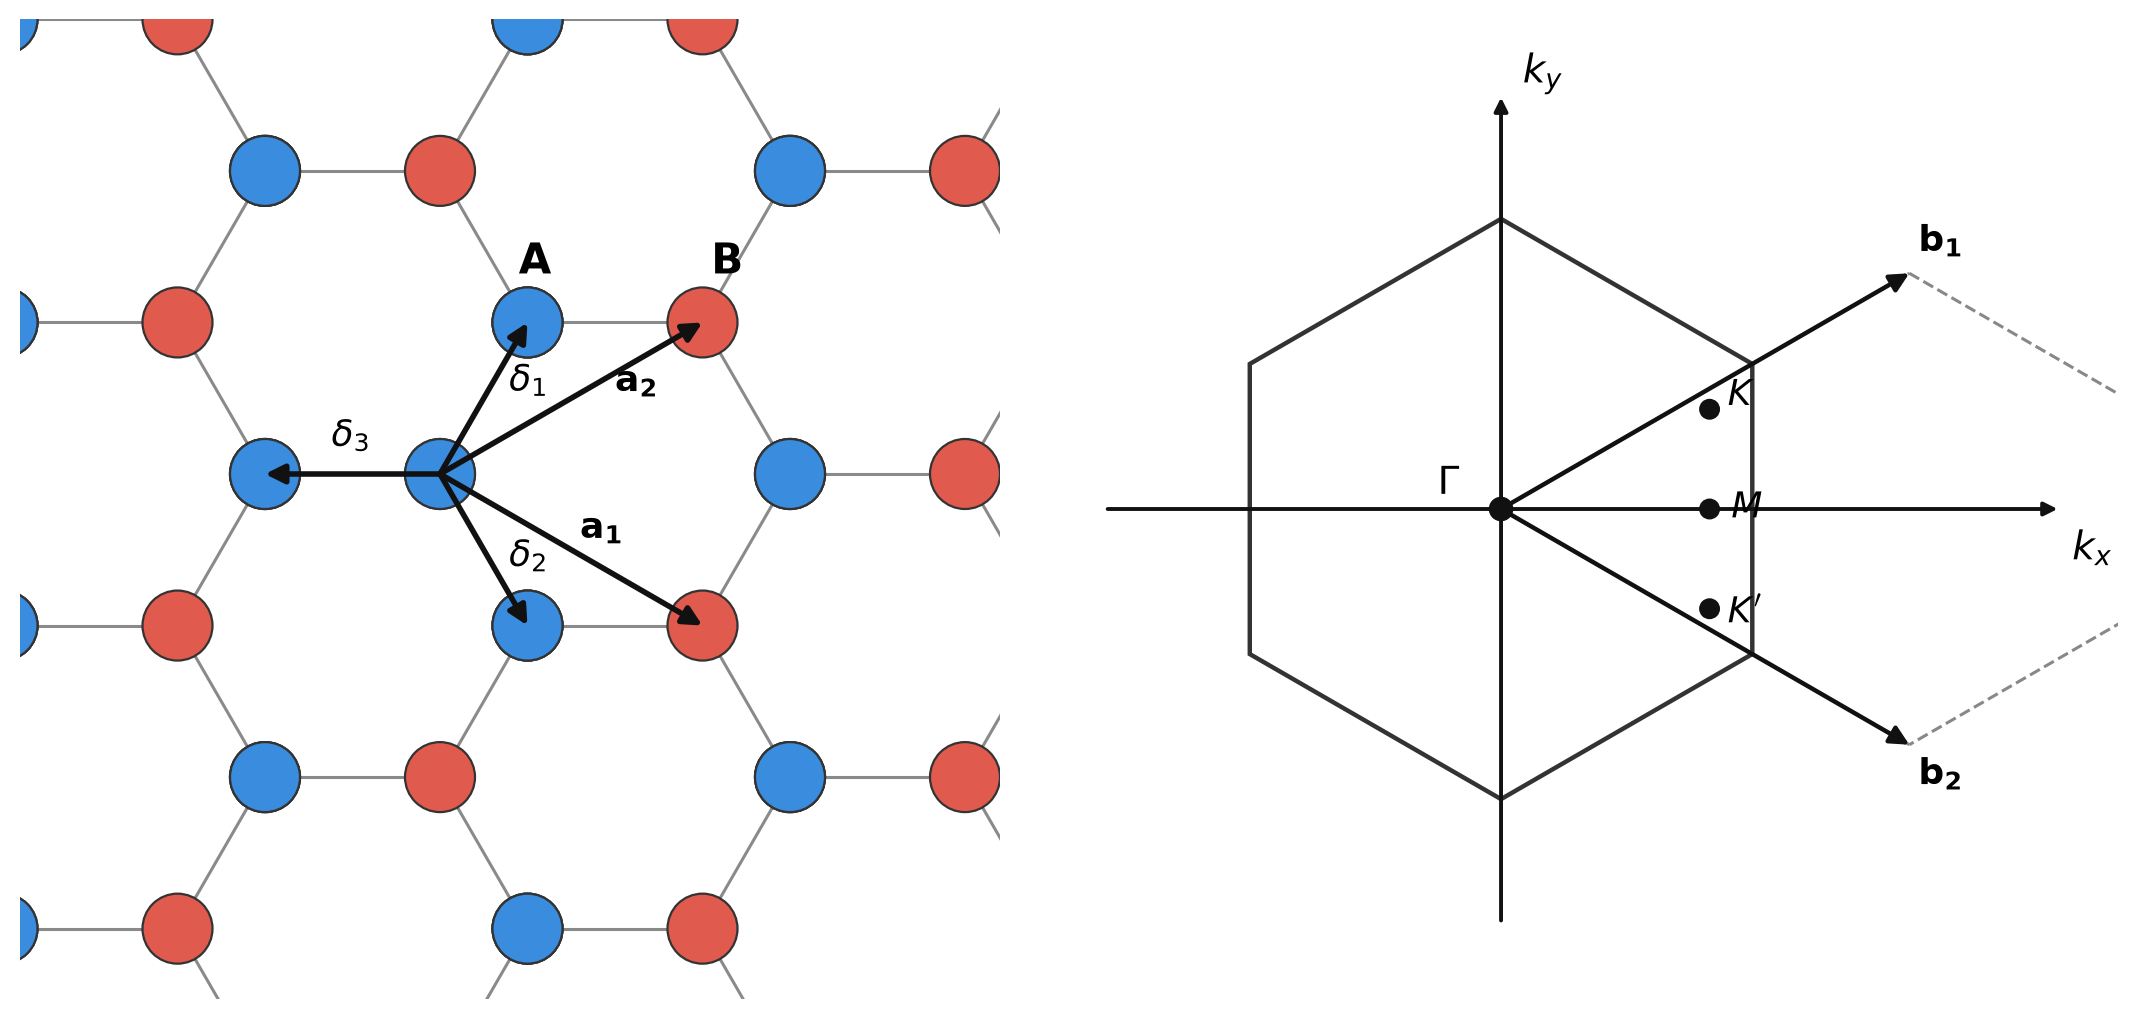
\includegraphics[width=0.8\textwidth]{Restyled graphene lattice and Brillouin zone.png}
    \caption{Graphene lattice and its Brillouin zone.~\cite{netoElectronicPropertiesGraphene2009}}
    \label{fig:graphene-lattice-bz}
\end{figure}

Given the above coordinate choice for graphene unit cell, the band structure of a (N,0) CNT (Zig-Zag CNT), obtained from the tight-binding model of graphene~\cite{netoElectronicPropertiesGraphene2009}, is expressed as 
(Obtained by putting the quantization condition $N a k_y = 2\pi m$ in the graphene band structure): 

\begin{equation}\label{eq:band-structure}
    E = \pm t_0 \sqrt{f(k_x, m)} = \pm t_0 \sqrt{1+4\cos\bigg{(}\frac{3k_xa}{2}\bigg{)}\cos\bigg{(}\frac{\pi m}{N}\bigg{)}+4\cos^2\bigg{(}\frac{\pi m}{N}\bigg{)} }
\end{equation}

% How does (N,M) CNT get represented in lean4
% The E-k relation derivation ? 

% How is insertion of each numerical value or approximation assertion handled?
where $t_0 = 2.5eV$ is the tight-binding coupling constant, where $a$ is the lattice constant and m is an index that runs from $0$ to $N-1$.
A thorough derivation can be found in~\cite{schonenbergerBandstructureGrapheneCarbon2015}, although with axes rotated.

\begin{figure}[ht]
    \centering
    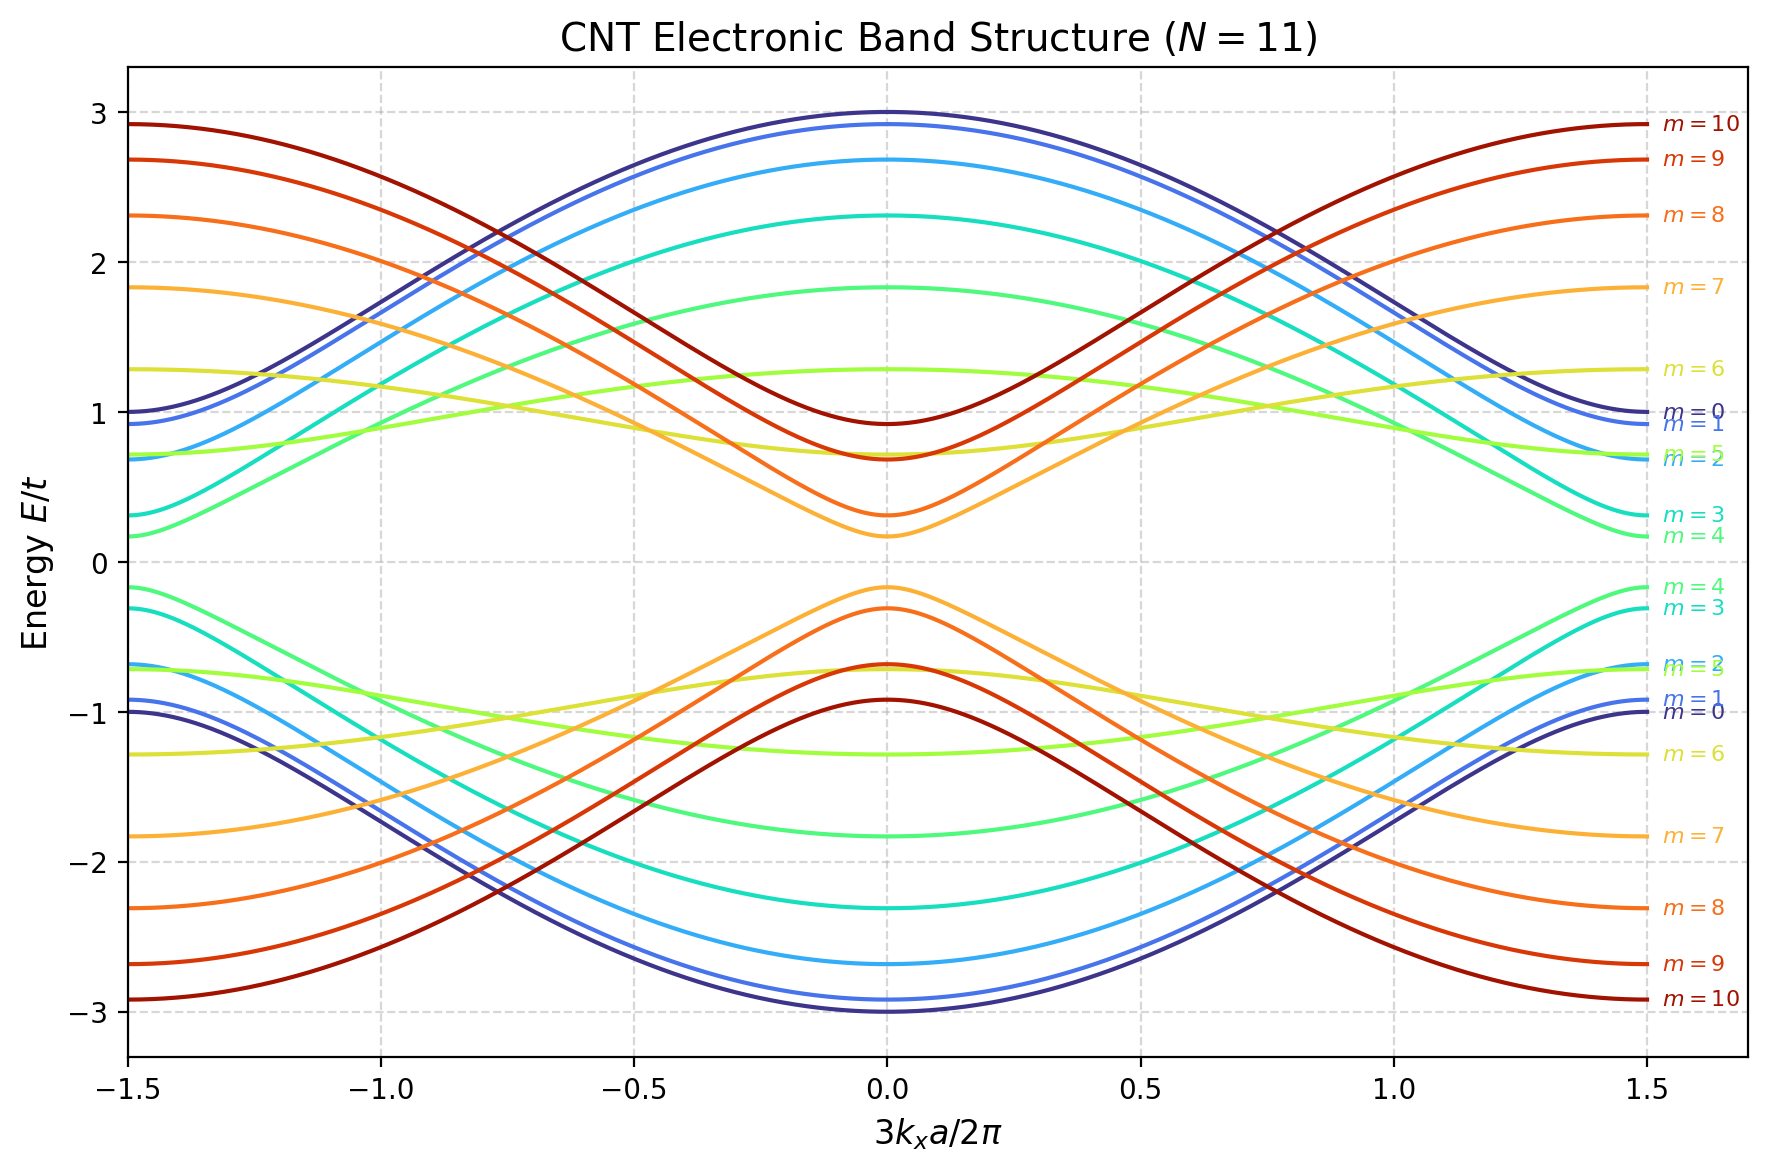
\includegraphics[width=0.8\textwidth]{cnt_band_structure_N11.png}
    \caption{Electronic band structure of an $N=11$ zig-zag CNT computed from~\eqref{eq:band-structure}, with each curve labelled by its sub-band index $m = 0, 1, \ldots, N-1$.}
    \label{fig:cnt-band-structure}
\end{figure}
\subsection{Analytical expression for band-gap}\label{sec:bandgap}
CNT is one of those nice systems where the band-gap can be expressed analytically.
In~\eqref{eq:band-structure}, consider the bands with a $+$ sign. Then
the band-minimum, $E_{min_m}$ for a given band index, $m$, occurs when
\begin{equation}
\partial_{k_x}f(k_x, m)=0 \implies \frac{3k_xa}{2} \in \{0,\pi\}
\end{equation}

while the minimum of the set $E_{min_m}$ across all bands, as $m$ is varied is obtained when the 
quadratic equation in $\cos(\frac{\pi m}{N})$ is minimized: 
\begin{equation}
\begin{split}
    \partial_{\cos(\pi m/N)}f(k_x, m)\bigg|_{\frac{3k_xa}{2} \in \{0,\pi\}} &= 0 \\
    \implies \cos\bigg(\frac{\pi m}{N}\bigg) &= -\frac{1}{2}\cos\bigg(\frac{3k_xa}{2}\bigg)\bigg|_{\frac{3k_xa}{2} \in \{0,\pi\}} \\
    &= \pm \frac{1}{2}
\end{split}
\end{equation}
 which means $\cos\bigg(\frac{\pi m}{N}\bigg)$ needs to be as close to $\pm\frac{1}{2}$ as possible. 
 This is exactly possible whenever $N = 3m$, then band-gap is exactly 0 and we call such a CNT metallic. 
 Though in this article, we will consider only CNTs with a bandgap so  
 let us restrict ourselves to when $N=3m-1$, i.e $N=8, 11, 14, 17$ etc. A representative
 band-diagram is shown for $N=11$ below: 
 

 Given a value of $N$, $m$ will take values in the set $\{0, 1, 2, \ldots, N-1\}$. Let
\[
    m_0 := \operatorname*{arg\,min}_{m} \left\{\left| m - \frac{N}{3} \right|, \left| m - \frac{2N}{3} \right|\right\}.
\]
The band-minima is then written as (pairing the value of $m_0$ with  $\frac{3k_x a}{2} = \pi /0$):
\begin{equation}\label{eq:bandgap}
    E_g = 2t_0\sqrt{1-4\cos\bigg{(}\frac{\pi m_0}{N}\bigg{)}+4\cos^2\bigg{(}\frac{\pi m_0}{N}\bigg{)} } .
\end{equation}

\subsection{Analytial expression for Density of States}
Good point to obtain an expression for the density of states near the band-minimum. 
First, we need to show the following approximation holds near the band-minimum:

\begin{equation}\label{eq:dkx-dE}
    \frac{d}{dE} \bigg{(}\frac{3k_x a}{2}\bigg{)} \approx \frac{|E|}{t_0\sqrt{E^2-(E_g/2)^2}}
\end{equation}



%What do we mean by DoS? We mean Density of States at energy E per unit length, so that it is an intensive quantity.
%The DoS can be written for the case of 1D CNT as:
%\begin{equation}
%    D(E) = \frac{1}{L}\frac{ \text{\# States in [k, k+dk]}}{dk(E)}
%\end{equation}

In section~\ref{sec:bandgap} we discovered that a neighbourhood of band minimum comprises of $m_0$ with $\frac{3k_x a}{2} \approx \pi$. 
So equation~\eqref{eq:band-structure} around band-minimum can be rewritten as a taylor expansion around $\frac{3k_x a}{2} = \pi$: 
(Hereafter, $k_x$ refers to the small-signal expansion around $k_x = \frac{2\pi}{3a}$)
\begin{equation}
    E \approx \pm t_0 \sqrt{1+4\cos\bigg{(}\frac{\pi m_0}{N}\bigg{)}\bigg{(}-1-\frac{1}{2}\bigg{(}\frac{3k_xa}{2}\bigg{)}^2\bigg{)}+4\cos^2\bigg{(}\frac{\pi m_0}{N}\bigg{)} }
\end{equation}
Plugging in the value of $E_g$ from~\eqref{eq:bandgap}, we get:

\begin{equation}
    E \approx \pm t_0 \sqrt{\bigg{(}\frac{E_g}{2t_0}\bigg{)}^2-\bigg{(}2\cos\bigg{(}\frac{\pi m_0}{N}\bigg{)}\bigg{)}\bigg{(}\frac{3k_xa}{2}\bigg{)}^2 }
\end{equation}

Since $m_0$ takes $\cos(\frac{\pi m_0}{N})$ to be as close to $\frac{1}{2}$ as possible,
for a big enough N, we can approximate the above equation as:

\begin{equation}
    E \approx \pm t_0 \sqrt{\bigg{(}\frac{E_g}{2t_0}\bigg{)}^2-\bigg{(}\frac{3k_xa}{2}\bigg{)}^2 }
\end{equation}
Rerrangment gives:

\begin{equation}\label{eq:kx-of-E}
    \frac{3k_xa}{2} \approx \pm \frac{1}{t_0}\sqrt{E^2 - \bigg{(}\frac{E_g}{2}\bigg{)}^2}
\end{equation}

\eqref{eq:dkx-dE} follows from differentiating~\eqref{eq:kx-of-E} with respect to $E$.


From here, the calculation of density of states is 
straightforward. Density of States is defined as:

\begin{equation}
    D(E) = \frac{1}{L}\frac{ \text{\# States in [E, E+ dE]}}{dE}
\end{equation}

For a periodic system, this means counting the number of values of $k_x$ whose energy lies in the 
range $[E, E+dE]$ i.e. $dk(E)$. We already know $dk(E)$ from ~\eqref{eq:dkx-dE}.

k-states are spaced uniformly with space 
\begin{equation}\label{eq:k-spacing}
    d \bigg{(}\frac{3k_x a}{2}\bigg{)} = \frac{3\pi a}{L}
\end{equation}

Now we compute $D(E)$ in steps, first we find the numerator ie \# states in [k, k+dk]:
\begin{equation}
    dk(E) = \frac{d}{dE} \bigg{(}\frac{3k_x a}{2}dE \bigg{)} \approx \frac{|E|dE}{t_0\sqrt{E^2-(E_g/2)^2}}
\end{equation}

The number of states in this range of $dk$ is given by dividing above equation by \ref{eq:k-spacing}
\begin{equation}
     \frac{1}{ \frac{3\pi a}{L}}\frac{d}{dE} \bigg{(}\frac{3k_x a}{2}dE \bigg{)} \approx \frac{1}{ \frac{3\pi a}{L}}\frac{|E|dE}{t_0\sqrt{E^2-(E_g/2)^2}}
\end{equation}
Dividing by L gives:
\begin{equation}
     D(E) \approx \frac{1}{3\pi a}\frac{|E|}{t_0\sqrt{E^2-(E_g/2)^2}}
\end{equation}

\subsubsection{Degeneracy}

But the equation above is not yet correct, since there is an eight-fold ($2 \times 2 \times 2$) degeneracy in a CNT:
\begin{enumerate}
    \item In~\eqref{eq:band-structure}, $(k_x, m)$ and $(-k_x, N-m)$ give the same energy (a factor of $2$).
    \item Electron spin takes two values (a factor of $2$).
    \item Each band is symmetric about its minimum, and our expression considered only a single branch of the expansion around the band-minimum (a factor of $2$).
\end{enumerate}


The last degeneracy can also be seen in the figure 2 in Introduction section.
The final Density of States is then given as:
\begin{equation}
     D(E) \approx \frac{8}{3\pi a}\frac{|E|}{t_0\sqrt{E^2-(E_g/2)^2}}
\end{equation}

\subsubsection{Verification}
Let us derive the surface charge density expression
Each state has its charge distributed uniformly across the cylinder.
So that the surface charge density is given as (remember DoS is already per unit length, 
so we just need to divide by the circumference of the cylinder while computing surface charge 
density):
\begin{equation}
    \sigma = \frac{q}{2\pi R}\int_{E_1}^{E_2} D(E)f(E)dE
\end{equation}

\begin{equation}
    \sigma = \int_{E_1}^{E_2} \frac{8q}{6\pi^2 R a}\frac{|E|}{t_0\sqrt{E^2-(E_g/2)^2}}f(E)dE
\end{equation}
From geometry, we know the relation:
\begin{equation}
    2R\sin\frac{\pi}{N} = \sqrt{3}a
\end{equation}
For big enough N, we can linearize sin function and this gives:
\begin{equation}
    \sigma = \int_{E_1}^{E_2} \frac{8q}{3\sqrt{3}\pi  a^2 N}\frac{|E|}{t_0\sqrt{E^2-(E_g/2)^2}}f(E)dE
\end{equation}
This agrees with the expression we have in Eq. 15 of ~\cite{leonardPropertiesShortChannel2006} 


% k-states are spaced uniformly with space $d \bigg{(}\frac{3k_x a}{2}\bigg{)} = \frac{3\pi a}{L}$ 

% Now we compute D(E) in steps. First we find the numerator ie \# states in [k, k+dk]:
% \begin{equation}
%      \frac{1}{ \frac{3\pi a}{L}}\frac{d}{dE} \bigg{(}\frac{3k_x a}{2}dE \bigg{)} \approx \frac{1}{ \frac{3\pi a}{L}}\frac{|E|dE}{t_0\sqrt{E^2-(E_g/2)^2}}
% \end{equation}
% Dividing by L gives:
% \begin{equation}
%      D(E) \approx \frac{1}{3\pi a}\frac{|E|}{t_0\sqrt{E^2-(E_g/2)^2}}
% \end{equation}
% But this equation is not correct since there is a degeneracy of 8: Degeneracy of 2 because of spins, degeneracy of 2 because there are two bands and each band has further even symmetry, so two branches to each band. Hence the DOS is actually given as:
% \begin{equation}
%      D(E) \approx \frac{8}{3\pi a}\frac{|E|}{t_0\sqrt{E^2-(E_g/2)^2}}
% \end{equation}

% (Need to prove there are two bands and that the only the lowest band comes into picture. This can be verified with the second level of approximation itself)

% \section{Surface Charge Density}
% Each state has its charge distributed uniformly across the cylinder.
% So that the surface charge density is given as (remember DoS is already per unit length, so that's automatically taken care of while computing surface charge density)
% \begin{equation}
%     \sigma = \frac{q}{2\pi R}\int_{E_1}^{E_2} D(E)f(E)dE
% \end{equation}

% \begin{equation}
%     \sigma = \int_{E_1}^{E_2} \frac{8q}{6\pi^2 R a}\frac{|E|}{t_0\sqrt{E^2-(E_g/2)^2}}f(E)dE
% \end{equation}
% From geometry, we know the relation:
% \begin{equation}
%     2R\sin\frac{\pi}{N} = \sqrt{3}a
% \end{equation}
% For big enough N, we can linearize sin function and this gives:
% \begin{equation}
%     \sigma = \int_{E_1}^{E_2} \frac{8q}{3\sqrt{3}\pi  a^2 N}\frac{|E|}{t_0\sqrt{E^2-(E_g/2)^2}}f(E)dE
% \end{equation}
% This agrees with the expression we have in~\cite{leonardPropertiesShortChannel2006} subject to the above mentioned constraints.

% Let us find the charge before ($\rho_i$) and after ($\rho_f$) thermal equilibrium is attained. Assume $D(E)$ is the density of states at energy E, $f(E, E_f)$ is the Fermi-Dirac distribution occupancy factor at energy E given fermi level energy at $E_f$ and after equilibrium has been attained, the CNT sits at an electrostatic potential of $V_0$, then:

% \begin{align}
%       \rho_f &= \int_{-\infty}^{\infty} D(E+V_0)f(E,E_f)\, dE \\
%       \rho_i &= \int_{-\infty}^{\infty} D(E)f(E, 0)\, dE
% \end{align}

% Here we assumed that before the two materials are brought close, the CNT has $E_f=0$ and after the CNT is charged to potential $V_0$, all the energy levels rise by $V_0$. The net charge accumulated by the CNT is then:

% \begin{align}
%       \delta \rho &= \rho_f-\rho_i \notag\\
%       &= \int_{-\infty}^{\infty} D(E+V_0)f(E,E_f)\, dE - \int_{-\infty}^{\infty} D(E)f(E, 0)\, dE \notag\\
%       &= \int_{-\infty}^{\infty} D(E)\bigl(f(E-V_0,E_f)-f(E,0)\bigr)\, dE
% \end{align}

% This equation represents the total charge as the sum of charge accumulated at each state in CNT due to the change of fermi level as seen by that state.
% Let us look now at the behaviour of the part of integrand made up of fermi functions:

% \begin{eqnarray}
% f(E-V_0,E_f)-f(E,0) = 0 \quad \forall E\geq \max(E_f+V_0, 0) +4\frac{kT}{q} \quad\text{and}\quad E\leq \min(E_f+V_0, 0) - 4\frac{kT}{q}
% \end{eqnarray}

% \section{Code}
% Check my github page

\bibliographystyle{unsrt}
\bibliography{references}





\end{document}
